\documentclass[11pt]{article}
\usepackage{amsmath}
\usepackage{graphicx}
\usepackage{physics}
\graphicspath{{img/}}

\begin{document}

\title{{\bf 11-755: MLSP}\\
       HW \#3: Clustering and EM}

\author{Nikolas Wolfe}

\date{December 15, 2015}
\maketitle


\section*{Problem 1: K-Means \& Spectral Clustering}
You are given a number of toy datasets. The visulized groud truth clustering configuration of these data: Aggregation (K=7), Bridge (K=2), Compound (K=6), Flame (K=2), Jain (K=2), Spiral (K=3) and TwoDiamond (K=2) are shown as follows:
\begin{center}
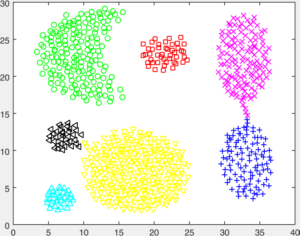
\includegraphics[scale=0.5]{aggregation}
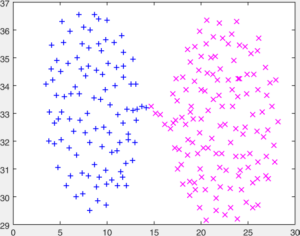
\includegraphics[scale=0.5]{bridge}
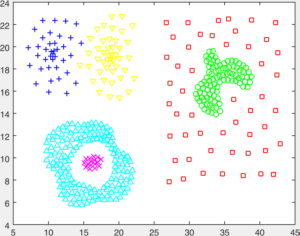
\includegraphics[scale=0.5]{compound}
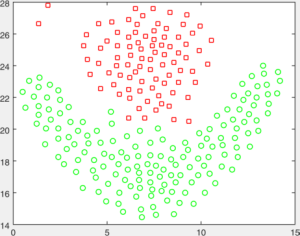
\includegraphics[scale=0.5]{flame}
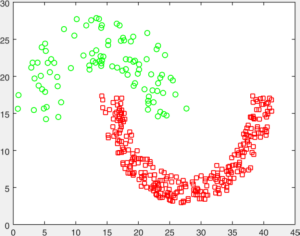
\includegraphics[scale=0.5]{jain}
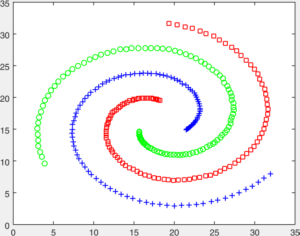
\includegraphics[scale=0.5]{spiral}
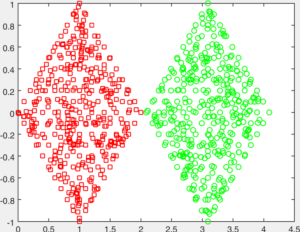
\includegraphics[scale=0.5]{twoDiamonds}
\end{center}
\pagebreak
{\bf Answer:}\\[5pt] 
I implemented this code in Java, using the Efficient Java Matrix Library (EJML) package to do matrix multiplication and Eigen/Singular Value decomposition. In general, spectral clustering works a lot better than K-means and is able to determine a lot of structure (such as the spiral pattern) that k-means is unable to find. 

In terms of evaluation, I ran the clustering algorithms and generated the confusion matrix between the most common label that emerges in each cluster and their actual labels. A diagonal matrix in this case is of course perfect performance. The accuracy can be determined from looking at the counts of labeled points for each class. 
\begin{center}\hspace*{-1.5cm}
	\begin{tabular}{| l | c | l |}
	\hline
	Dataset & Optimal K & Group Counts  \\ 
	\hline
  Aggregation & 7 & $[K_1, K_2, K_3, K_4, K_5, K_6, K_7] = [45, 170, 102, 273, 34, 130, 34]$\\
  	\hline
  	  Compound & 6 & $[K_1, K_2, K_3, K_4, K_6] = [50, 92, 38, 45, 158, 16]$ \\
  	  \hline
  	    Spiral & 3 & $[K_1, K_2, K_3] = [101, 105, 106]$ \\
  	    \hline
  Bridge & 2 & $[K_1, K_2] = [102, 13]$\\
  	\hline
  Flame & 2 & $[K_1, K_2] = [87, 153]$ \\
  	\hline
  Jain & 2 & $[K_1, K_2] = [276, 97] $\\
  	\hline
   Two Diamonds & 2 & $[K_1, K_2] = [400, 400]$ \\
  	\hline
	\end{tabular}
\end{center}\vspace*{0.5cm}
With this information, we can directly evaluate the quality of the Spectral and K-means clustering algorithms by simply comparing the diagonal of their confusion matrices (most common group label vs. actual label) to the vectors listed above above.
To run the java package, simply run the following from the root of this project:
\begin{verbatim}
java -jar nwolfe_hw3.jar 
\end{verbatim}
This will run the main method in the class \texttt{ClusterDriver.java}, which will then iterate through a small range of $\sigma$ values which are known to produce generally good spectral clusters, though it is often the case that several random restarts are required in order for the spectral clustering algorithm to settle into the optimal cluster groupings. In this report the best clusters have been chosen, though it is the case that when \textit{you} run it, it might produce an optimal grouping.

This code also produces the results as expected by the provided MATLAB scripts as CSV files in the root directory in which the jar is run. To generate the visualizations of the data, you may select the individual files you want and use the \texttt{visualize.m} script as provided. Alternatively, you may use the results I have included in the report and simply go to the \texttt{external} folder and run the \texttt{gen\_all\_figs.m} script.
\begin{verbatim}
cd external/
matlab gen_all_figs.m
\end{verbatim}
Alternatively, you could just look at the pictures in this here report. That's probably easier. 

\subsection*{Questions}
In your report, answer the following questions: 
\begin{enumerate}
\item Is the objective function of k-means a convex one?
\\[5pt] {\bf Answer:} The objective function which we are trying to minimize is the sum of Euclidean distances from each cluster centroid to each cluster datapoint. However, the number of clusters $K$ is discrete, which means we cannot take the derivative of this function and determine the optimal grouping (i.e. the minimum distance sum over all clusters) either analytically or through gradient descent or some other minimization technique. (This is also the case for spectral clustering.) Furthermore, the 2nd derivative of the Euclidean distance function is not zero. Because there is no way to find the optimal grouping (and perhaps no grouping actually exists), this is not a convex optimization problem. 

\item Can the iterative updating scheme in k-means return a solution which achieves the global minimum of the k-means objective function?
\\[5pt] {\bf Answer:} Newp. No. Sorry! As stated above, there is no guaranteed minimum for the objective function because it isn't convex. There may be an infinite number of viable ways to cluster the data. 
\item If yes, why? If not, why not and are there any practical ways to partially fix this?
\\[5pt] {\bf Answer:} One of the ways to fix this is, first off, to attempt to pick the initialization of the cluster centroids according to some logic. In this case we happen to know the optimal value of $K$ from the labeled data. This may result in a better teasing apart of the datapoints and less moving around before the algorithm converges. Another way might be to use bottom up or top down clustering, i.e. to start with a single cluster containing all the data, perturb the centroid and then continually break the clusters apart until an optimal value of $K$ is reached. Or we could start with a large number of clusters and then continually merge them according to some criteria until we reach a desired value of $K$. 
\end{enumerate}
\subsection*{Results}
For each problem I have printed the output of the algorithm after a single run. At the beginning of each section is a comparison of 3 pictures. 
\subsubsection*{Aggregation} 
From left to right, the images are:
\begin{enumerate}
\item Ground Truth
\item Spectral Clustering Result
\item K-Means Clustering Result
\end{enumerate}
\begin{center}
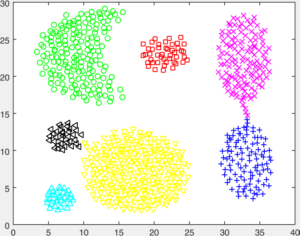
\includegraphics[scale=0.5]{aggregation} \ 
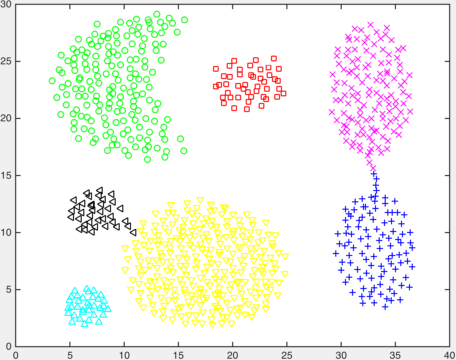
\includegraphics[scale=0.25]{results_spectral_aggregation} \ 
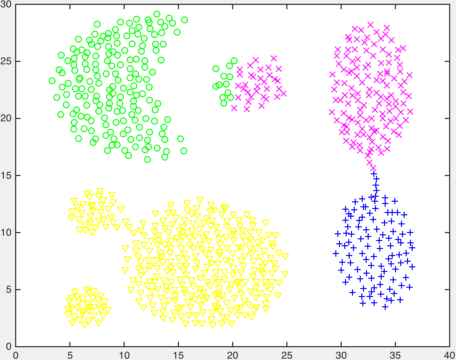
\includegraphics[scale=0.25]{results_kmeans_aggregation}
\end{center}
\textbf{Aggregation: Spectral Clustering}
\begin{verbatim}
Reading data values in data/Aggregation.csv...
Reading data values in data/Bridge.csv...
Reading data values in data/Compound.csv...
Reading data values in data/Flame.csv...
Reading data values in data/Jain.csv...
Reading data values in data/Spiral.csv...
Reading data values in data/TwoDiamonds.csv...

=============== AGGREGATION: SPECTRAL CLUSTERING ===============
With sigma = 0.47

label  1    2    3    4    5    6    7  
___________________________________________________________
1 |    45   0    0    0    0    0    0  
2 |    0    170  0    0    0    0    0  
3 |    0    0    1    0    0    0    0  
4 |    0    0    0    270  0    0    0  
5 |    0    0    0    0    34   0    0  
6 |    0    0    101  0    0    130  0  
7 |    0    0    0    3    0    0    34  

With sigma = 0.48

label  1    2    3    4    5    6    7   
___________________________________________________________
1 |    45   0    0    0    0    0    0   
2 |    0    170  0    0    0    0    0   
3 |    0    0    102  0    0    2    0   
4 |    0    0    0    270  0    0    0   
5 |    0    0    0    0    34   0    0   
6 |    0    0    0    0    0    128  0   
7 |    0    0    0    3    0    0    34   

With sigma = 0.49

... Output truncated ... 
\end{verbatim}
In the second run above, the diagonal is almost perfect, save for a few items misplaced in groups 3 and 7. 
\\[5pt]
\textbf{Aggregation: K-Means Clustering} 
\begin{verbatim}
===================== AGGREGATION: K MEANS =====================

label  1    2    3    4    5    6    7    
___________________________________________________________
1 |    0    0    0    0    0    0    0    
2 |    17   170  0    0    0    0    0    
3 |    0    0    102  0    0    3    0    
4 |    0    0    0    273  34   0    34    
5 |    0    0    0    0    0    0    0    
6 |    28   0    0    0    0    127  0    
7 |    0    0    0    0    0    0    0    

----------------------------------------------------------
\end{verbatim}
In the k-means clustering it's clear that several groups did not even emerge from the data (though this does not mean they were empty.)
\\[5pt]
\subsubsection*{Bridge} 
From left to right, the images are:
\begin{enumerate}
\item Ground Truth
\item Spectral Clustering Result
\item K-Means Clustering Result
\end{enumerate}
\begin{center}
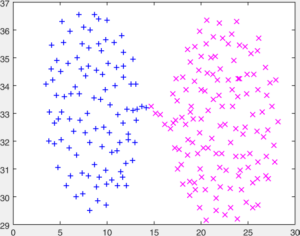
\includegraphics[scale=0.5]{bridge} \ 
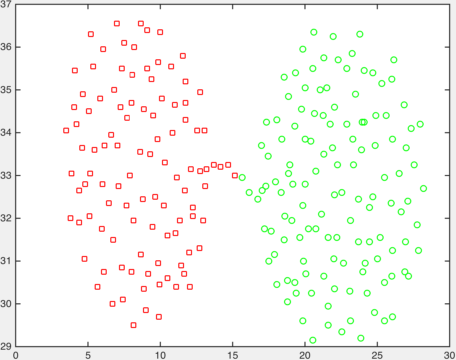
\includegraphics[scale=0.25]{results_spectral_bridge} \ 
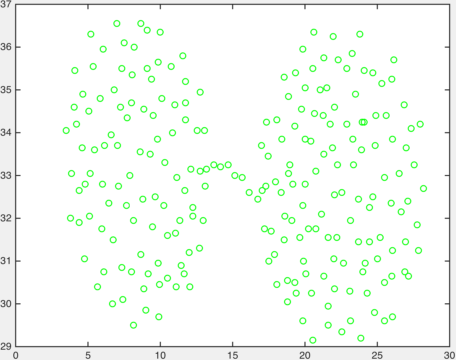
\includegraphics[scale=0.25]{results_kmeans_bridge}
\end{center}
\textbf{Bridge: Spectral Clustering} 
\begin{verbatim}

=============== BRIDGE: SPECTRAL CLUSTERING ===============
With sigma = 0.42

... Output truncated ... 	

With sigma = 0.44

label    1    2    
___________________
1 |      102  2    
2 |      0    128    

With sigma = 0.45

label    1    2    
___________________
1 |      58   58    
2 |      44   72    

\end{verbatim}
In one case the grouping was nearly perfect, and in another the data was more or less spread around a different kind of grouping.
\\[5pt]
\textbf{Bridge: K-Means Clustering} 
\begin{verbatim}
===================== BRIDGE: K MEANS =====================

label    1    2    
___________________
1 |      0    0    
2 |      102  130    

----------------------------------------------------------
\end{verbatim}
Again, K-means was not able to find the right clustering... 
\\[5pt]

\subsubsection*{Compound} 
From left to right, the images are:
\begin{enumerate}
\item Ground Truth
\item Spectral Clustering Result
\item K-Means Clustering Result
\end{enumerate}
\begin{center}
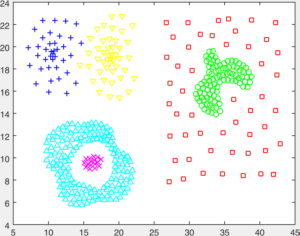
\includegraphics[scale=0.5]{compound} \ 
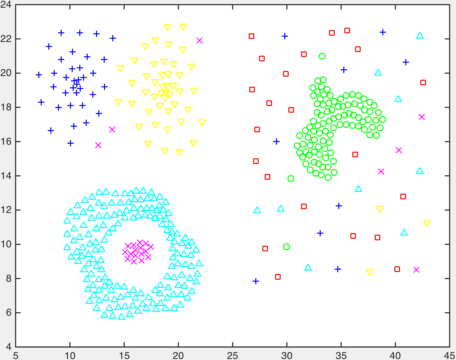
\includegraphics[scale=0.25]{results_spectral_compound} \ 
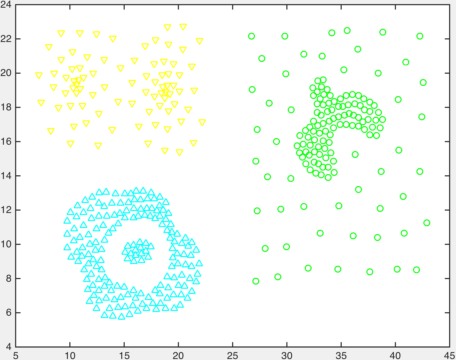
\includegraphics[scale=0.25]{results_kmeans_compound}
\end{center}

\textbf{Compound: Spectral Clustering} 
\begin{verbatim}

=============== COMPOUND: SPECTRAL CLUSTERING ===============

With sigma = 0.154

label  1    2    3    4    5    6    
___________________________________________________
1 |    21   0    1    1    0    0    
2 |    6    92   0    0    0    0    
3 |    12   0    33   0    0    0    
4 |    3    0    1    44   0    0    
5 |    5    0    2    0    158  0    
6 |    3    0    1    0    0    16    

With sigma = 0.155

label  1    2    3    4    5    6    
___________________________________________________
1 |    20   0    2    1    0    0    
2 |    6    92   1    44   0    0    
3 |    11   0    35   0    0    0    
4 |    0    0    0    0    0    0    
5 |    7    0    0    0    158  0    
6 |    6    0    0    0    0    16    

... Output truncated ... 	

\end{verbatim}
This grouping is particularly interesting because the groups in the compound picture were very difficult to tease apart, and yet we see here a diagonal clearly taking shape, except for some overlap with group 1.
\\[5pt]
\textbf{Compound: K-Means Clustering} 
\begin{verbatim}
===================== COMPOUND: K MEANS =====================

label  1    2    3    4    5    6    
___________________________________________________
1 |    0    0    0    0    0    0    
2 |    48   92   0    0    0    0    
3 |    0    0    38   1    0    0    
4 |    2    0    0    44   0    0    
5 |    0    0    0    0    158  16    
6 |    0    0    0    0    0    0    

----------------------------------------------------------

\end{verbatim}

\subsubsection*{Flame} 
From left to right, the images are:
\begin{enumerate}
\item Ground Truth
\item Spectral Clustering Result
\item K-Means Clustering Result
\end{enumerate}
\begin{center}
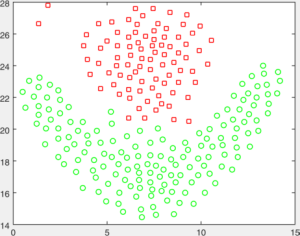
\includegraphics[scale=0.5]{flame} \ 
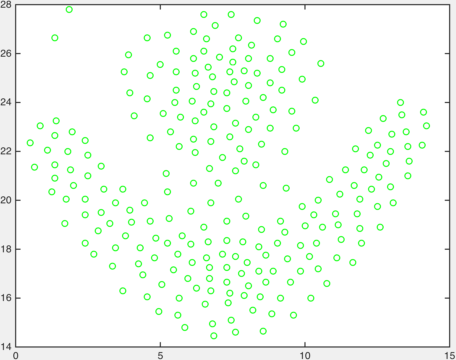
\includegraphics[scale=0.25]{results_spectral_flame} \ 
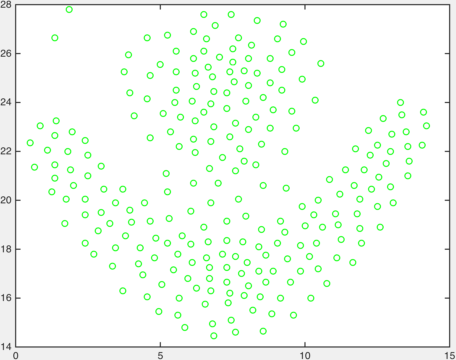
\includegraphics[scale=0.25]{results_kmeans_flame}
\end{center}


\textbf{Aggregation: Flame Clustering} 
\begin{verbatim}
=============== FLAME: SPECTRAL CLUSTERING ===============
With sigma = 0.735

label    1    2    
___________________
1 |      0    0    
2 |      87   153    

\end{verbatim}
\textbf{Flame: K-Means Clustering} 
\begin{verbatim}
===================== FLAME: K MEANS =====================

label    1    2    
___________________
1 |      0    0    
2 |      87   153    

----------------------------------------------------------

\end{verbatim}
\subsubsection*{Jain} 
From left to right, the images are:
\begin{enumerate}
\item Ground Truth
\item Spectral Clustering Result
\item K-Means Clustering Result
\end{enumerate}
\begin{center}
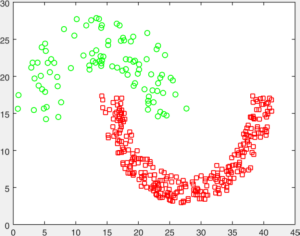
\includegraphics[scale=0.5]{jain} \ 
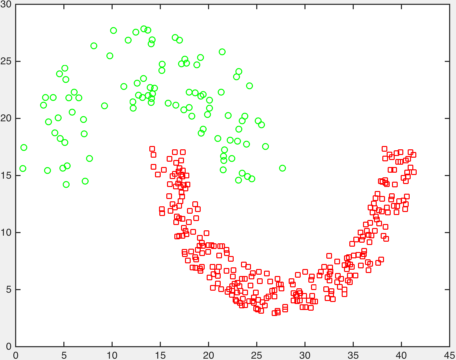
\includegraphics[scale=0.25]{results_spectral_jain} \ 
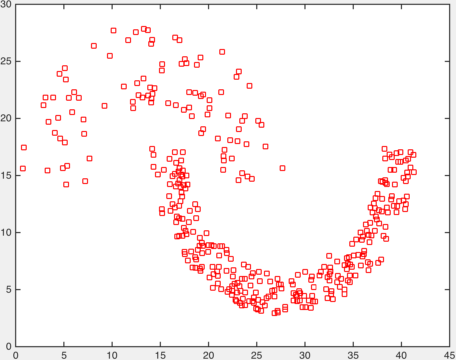
\includegraphics[scale=0.25]{results_kmeans_jain}
\end{center}
\textbf{Jain: Spectral Clustering} 
\begin{verbatim}
=============== JAIN: SPECTRAL CLUSTERING ===============

With sigma = 0.303

label    1    2    
___________________
1 |      276  0    
2 |      0    97    

With sigma = 0.304

label    1    2    
___________________
1 |      276  97    
2 |      0    0    

... Output truncated ... 	

\end{verbatim}
\textbf{Jain: K-Means Clustering} 
\begin{verbatim}

===================== JAIN: K MEANS =====================

label    1    2    
___________________
1 |      276  97    
2 |      0    0    

----------------------------------------------------------

\end{verbatim}

\subsubsection*{Spiral} 
From left to right, the images are:
\begin{enumerate}
\item Ground Truth
\item Spectral Clustering Result
\item K-Means Clustering Result
\end{enumerate}
\begin{center}
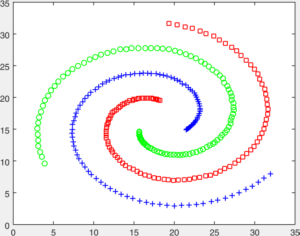
\includegraphics[scale=0.5]{spiral} \ 
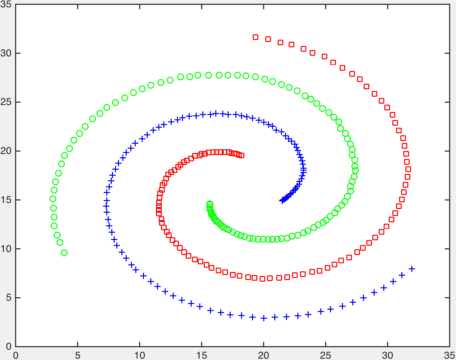
\includegraphics[scale=0.25]{results_spectral_spiral} \ 
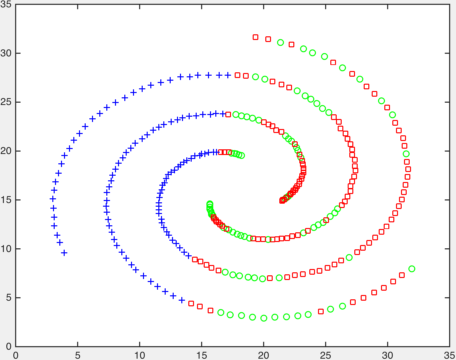
\includegraphics[scale=0.25]{results_kmeans_spiral}
\end{center}

\textbf{Spiral: Spectral Clustering} 
\begin{verbatim}

=============== SPIRAL: SPECTRAL CLUSTERING ===============
With sigma = 0.2

label  1    2    3    
___________________________
1 |    101  0    0    
2 |    0    105  0    
3 |    0    0    106    

With sigma = 0.30000000000000004

label  1    2    3    
___________________________
1 |    101  0    0    
2 |    0    105  0    
3 |    0    0    106    

With sigma = 0.4

label  1    2    3    
___________________________
1 |    101  0    0    
2 |    0    105  0    
3 |    0    0    106    

... Output truncated ... 	

\end{verbatim}
Given the shape in this case we can really see the difference between spectral clustering and k-means. This grouping was found perfectly, all zeros in the off-diagonal elements, with even a variable number of settings for $\sigma$. Looking at the k-means result below, it's clear that there's a real distinction here.
\\[5pt]
\textbf{Spiral: K-Means Clustering} 
\begin{verbatim}

===================== SPIRAL: K MEANS =====================

label  1    2    3    
___________________________
1 |    66   54   53    
2 |    0    0    0    
3 |    35   51   53    

----------------------------------------------------------

\end{verbatim}

\subsubsection*{Two Diamonds} 
From left to right, the images are:
\begin{enumerate}
\item Ground Truth
\item Spectral Clustering Result
\item K-Means Clustering Result
\end{enumerate}
\begin{center}
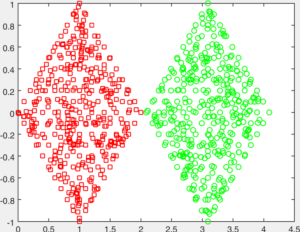
\includegraphics[scale=0.5]{twoDiamonds} \ 
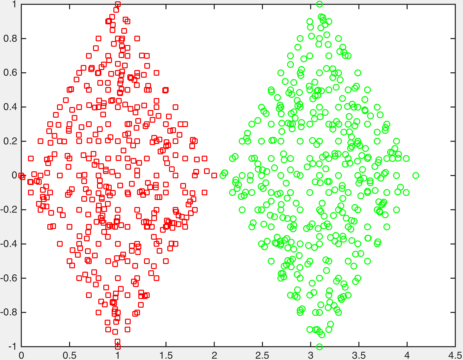
\includegraphics[scale=0.25]{results_spectral_two_diamonds} \ 
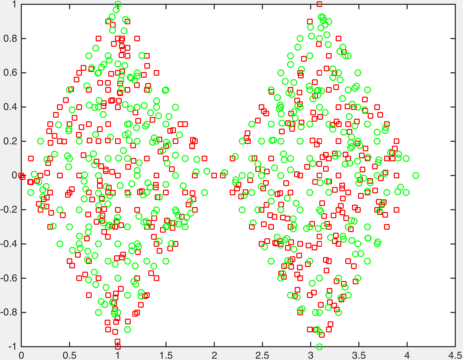
\includegraphics[scale=0.25]{results_kmeans_two_diamonds}
\end{center}
In the above case it appears that the two centroids in the k-means cluster were positioned in such a way that the points are ambiguously scattered, although I should note that I did not control for bad k-means results... I have only tried to present the best spectral clustering results because they're more fun anyway. 
\\[5pt]
\textbf{Two Diamonds: Spectral Clustering} 
\begin{verbatim}
=============== TWO DIAMONDS: SPECTRAL CLUSTERING ===============
With sigma = 20.0

label    1    2    
___________________
1 |      400  0    
2 |      0    400    

With sigma = 21.0

label    1    2    
___________________
1 |      204  198    
2 |      196  202    

... Output truncated ... 	

\end{verbatim}
\textbf{Two Diamonds: K-Means Clustering} 
\begin{verbatim}
===================== TWO DIAMONDS: K MEANS =====================

label    1    2    
___________________
1 |      203  196    
2 |      197  204    

----------------------------------------------------------
\end{verbatim}
\textbf{Questions \& Conclusion}
\\[5pt]
Compare your spectral clustering results with k-means. It is natural that on certain hard toy examples, both method won't generate perfect results? In your report, briefly analyze what is the advantage or disadvantage of spectral clustering over k-means. Why it is the case? 
\\[5pt]\textbf{Answer:}\\[5pt]
It is natural in the sense that the Gaussian kernel function used in spectral clustering is good at separating certain kinds of data and not others. Clearly separable groups, even if they have complicated boundaries (such as the spiral) are

Overall, I found that SVD was better at finding the basis vectors for the projection of the points into $k$ dimensional space. Furthermore in many cases it required a lot of random restarts before the groups coalesced into something reasonable. 
%\pagebreak
\section*{Problem 2: Expectation Maximization}

Let $Z$ be the sum of two random variables $X$ and $Y$, $(Z=X+Y)$, where $X$ and $Y$ are drawn independently from below discrete probability distributions with probability mass functions defined as:
\begin{align}
P(X=n) &= P_1(1-P_1)^{n-1}\\
P(Y=n) &= P_2(1-P_2)^{n-1}
\end{align}
Given samples of $Z$, derive an EM algorithm to estimate $P_1$ and $P_2$.
\\[5pt]\textbf{Answer:}
We have two discrete probability distributions. Samples of $Z$ are always the sum of $X$ and $Y$, so $Z$ is a multinomial distribution. We want to use the EM algorithm to estimate the maximum likelihood values of $P_1$ and $P_2$ that generated the samples of $Z$. We don't know $P_1$ and $P_2$ from observing $Z$, so we have to iteratively \textit{fractionate} the observations and reestimate our expectation for the values of $P_1$ and $P_2$.

There will be two steps in defining this EM algorithm: The E-step and the M-step. In the E-step, we compute an expectation for the data in $Z$ for the current (or assumed) values of $P_1$ and $P_2$. In the M-step, we treat this value as the ground truth and update the maximum likelihood values of $P_1$ and $P_2$. Overall, we are attempting to optimize the auxiliary function:
\begin{align}
Q(\theta, \theta^{\prime}) = \sum_H  \ P(H|Z,\theta^{\prime}) \ log(P(H,Z | \theta))
\end{align}
$H$ is the unseen variable (or variables)... In this case, $H$ represents the two hidden variables $X$ and $Y$, and $Z$ is the observation. $\theta$ represents the current values of the estimates of the model parameters (i.e. $P_1$ and $P_2$), and $\theta^{\prime}$ represents the values in the previous iteration of the algorithm.

This is just like the dice problem we solved in class. Given counts $c_1, c_2, c_3\ldots c_n$ for each discrete value of $n$ that $X$ and $Y$ take on, we can first calculate the total log probability of $P_1$ and $P_2$. (We will use log probability in this case because eventually we'll be taking the derivative to get the maximum likelihood value for $P_1$ and $P_2$ and the log is easily differentiable whereas this function as is totally sucks.)

The total log probabilities of $X$ and $Y$ are the sum of the probabilities of each value of $n$ times the counts $c_n$. This is:

\begin{align}
log(P(X)) &= \sum_n c_n \ log(P_1)  + log(1 - P_1)(n - 1) \\
log(P(Y)) &= \sum_n c_n \ log(P_2)  + log(1 - P_2)(n - 1)
\end{align}

To find the maximum likelihood values of $P_1$ and $P_2$ we differentiate this equation and set it to zero:

\begin{align}
\pdv{}{P_1}log(P(X)) &= \pdv{}{P_1}\left(\sum_n c_n \ log(P_1)  + log(1 - P_1)(n - 1)\right) \\
0 &= \pdv{}{P_1}\left(\sum_n c_n \ log(P_1)  + log(1 - P_1)(n - 1)\right) \\
0 &= \frac{c_n}{P_1}  - \frac{n - 1}{(1 - P_1)}\\
\frac{c_n}{P_1}  &= \frac{n - 1}{(1 - P_1)}\\
P_1 &= \frac{c_n}{c_n + n - 1}
\end{align}
Likewise for $P_2$:
\begin{align}
P_2 &= \frac{c_n}{c_n + n - 1}
\end{align}
For the first estimates of $P_1$ and $P_2$, we sum this value over all counts of $n$ in $Z$. Unfortunately, $Z$ represents the sum of two hidden variables $X$ and $Y$, and we do not know what values they actually take. Because we do not know, we fractionate the value of $Z$ into two bins, each of which can take on $n$ values. As we already know:
\begin{align}
Z = X + Y 
\end{align}
Every $Z$ \textit{must} contain a discrete $X$ and $Y$ value. Thus the values of $X$ and $Y$ represent \textit{fractions} of $Z$ implicitly. By fractionating $Z$, we get possible $X$ and $Y$ values directly. $X$ and $Y$ are the hidden variables, dependent on $P_1$ and $P_2$, and $Z$ is the observation. From the perspective of just $X$, the log likelihood for a given $n$ is:
\begin{align}
log(P(X = n | Z))
\end{align}
Which can be computed using Bayes' Rule:
\begin{align}
log(P(X = n | Z)) &= log(P(Z | X = n)) + log(P(X = n)) - log(P(Z)) \\
log(P(X = n | Z)) &= log(P(Z | X = n)) + log(P(X = n)) + Const
\end{align}
We have $log(P(X = n))$ from above:
\begin{align}
log(P(X = n)) &= log(P_1)  + log(1 - P_1)(n - 1)
\end{align}
The constant value we can typically ignore, and the value of $P(Z | X = n)$ we will compute by counting the values in 
\end{document}